\subsection{Circuito B}

Dopo aver eseguito in maniera preliminare le misure richieste, abbiamo deciso di semplificare il circuito per tenere sotto controllo le criticità descritte nella sezione precedente.

\subsubsection{Descrizione del circuito}

Il nuovo circuito segue lo schema in \autoref{circuitone} in basso.
I segnali dei PMT vengono inviati ai discriminatori per ottenere i segnali logici e agli attenuatori per essere poi inviati all'ADC. I segnali logici attraversano un modulo di antiretrigger per poi essere usati come trigger di acquisizioni singole o per effettuare coincidenze. Una copia dei segnali finisce al contatore. Abbiamo usato il timer per far partire/fermare le acquisizioni come abbiamo fatto per il circuito precedente.

\subsubsection{Problemi riscontrati}
\label{ref}
Dopo aver acceso l'apparato il bit stuck è scomparso
(probabilmente era dovuto a un mancato contatto nel modulo \texttt{CAMAC})
e l'aumento di risoluzione ci ha permesso di notare un problema che era già presente nel circuito precedente.
Abbiamo iniziato a vedere uno sdoppiamento dello spettro, come evidenziato dalla \autoref{doppio} sinistra. 

\begin{figure}
\centering
\subfloat
{
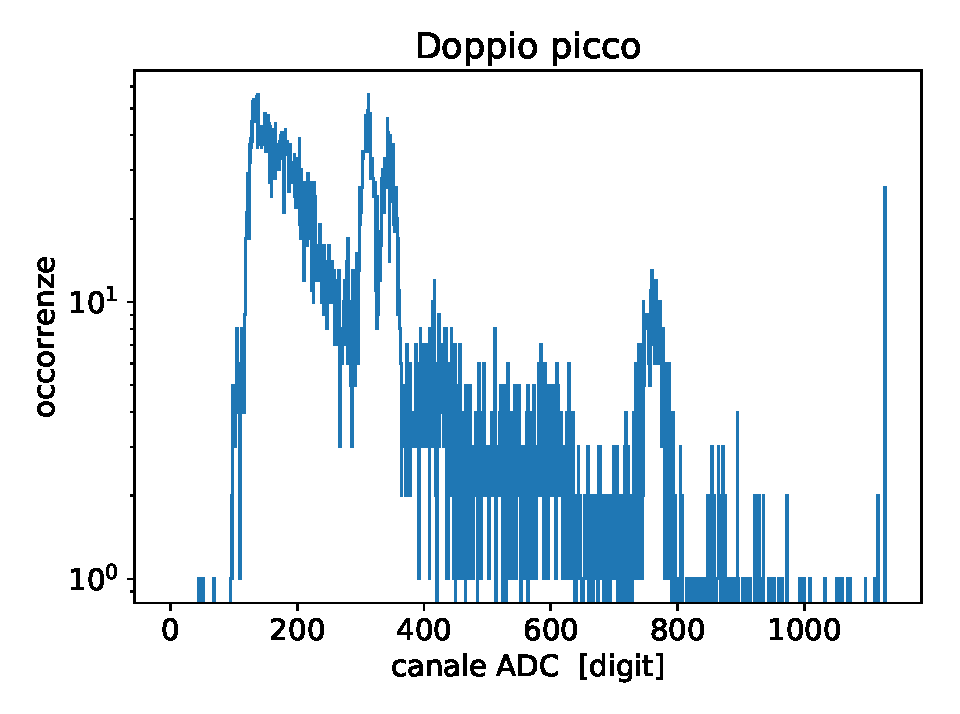
\includegraphics[width=18 em]{immagini/doppio}
}
\subfloat
{
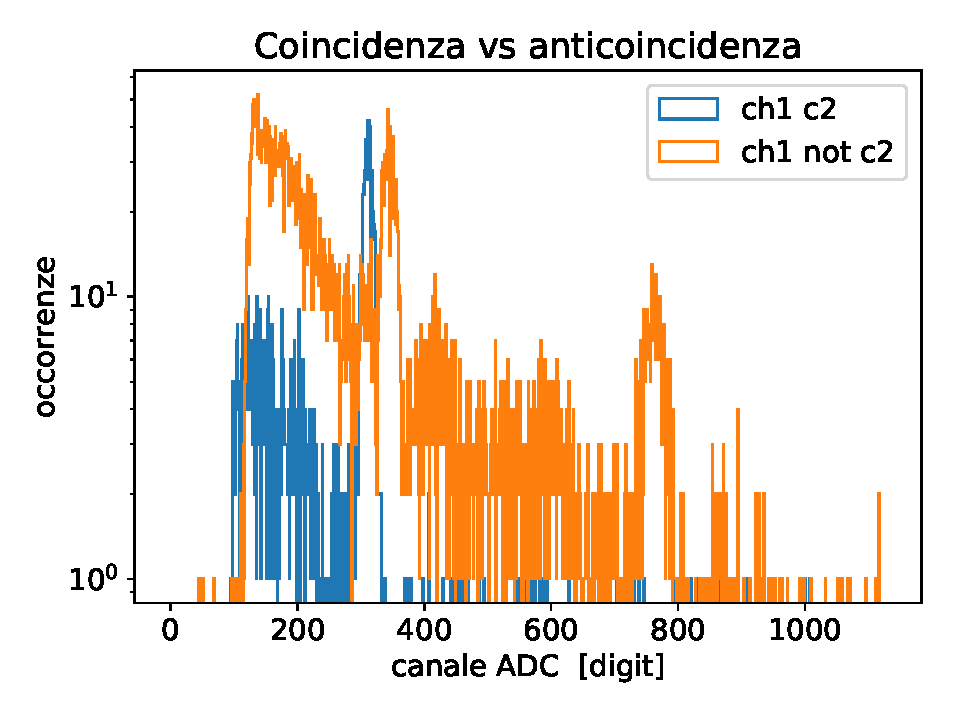
\includegraphics[width=18 em]{immagini/sdoppio}
}
\caption{A sinistra: acquisizione in cui l'annichilazione presenta due picchi.
A destra: divisione degli stessi dati in coincidenze (``c2'') e anticoincidenze (``not c2'').}
\label{doppio}
\end{figure}

Abbiamo poi scoperto la causa del problema, ovvero il crosstalk nell'ADC.
Come mostra il grafico di \autoref{doppio} destra, il doppio picco è la somma di quello osservato negli eventi in coincidenza con quello osservato in anticoincidenza,
ovvero in cui scatta il trigger del rivelatore 1 (quello su cui triggeriamo per salvare i dati) ma non quello del rivelatore 2.



\begin{figure}
\centering
\subfloat
{
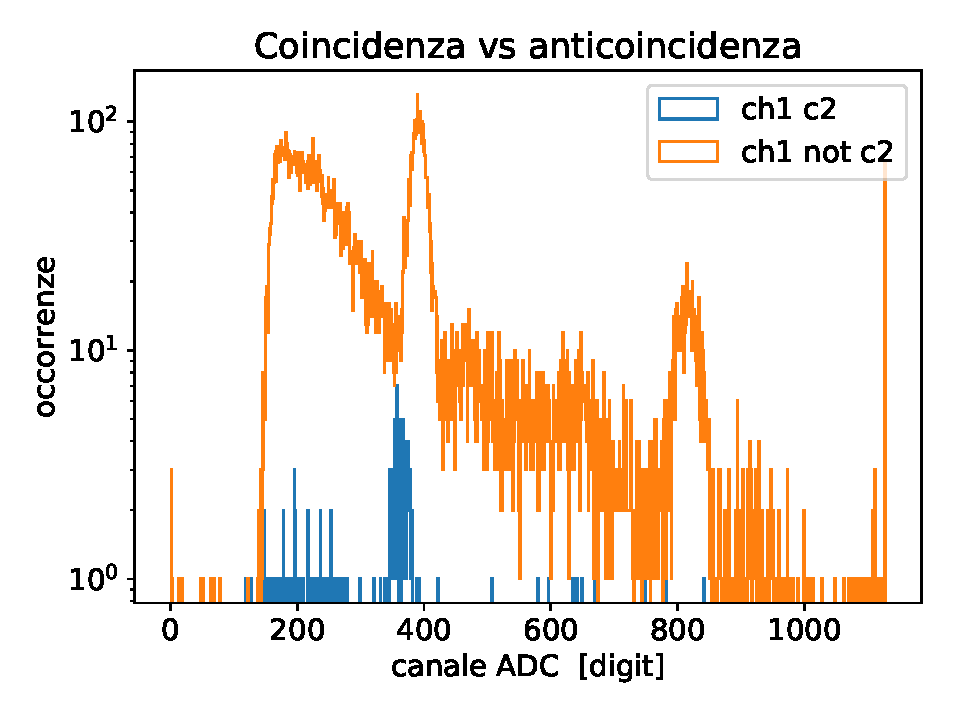
\includegraphics[width=20 em]{immagini/dist}
}
\caption{Grafico in cui il PMT1 è vicino alla sorgente mentre il PMT2 è lontano dalla sorgente.}
\label{sdoppio}
\end{figure}

Siamo arrivati alla conclusione che si tratti di un crosstalk dal fatto che il picco in anticoincidenza coincide con quello di un singolo canale quando tutti gli altri sono scollegati.
Inoltre abbiamo visto, aumentando la distanza di un PMT dalla sorgente, che il picco delle coincidenze si rimpicciolisce (perché ha meno eventi) e il picco in anticoincidenza tende ad assomigliare sempre di più a quello dell'acquisizione con canale singolo (\autoref{sdoppio});
questo permette di convincersi della causa anche senza separare gli eventi come in \autoref{doppio}.

Tale problema non era visibile ad occhio nudo nelle precedenti acquisizioni, ma un fit eseguito in seguito su misure ad alta statistica ha mostrato che il picco era modellato bene da due gaussiane ma non da una.

In seguito abbiamo provato che questo problema si riscontra anche quando i canali da analizzare non sono collegati ad ingressi adiacenti dell'ADC. Inspiegabilmente, il problema si è ripresentato solo a giorni alterni. 
